\chapter{Homework 1}
\section{}
Consider backward-Euler differencing and trapezoidal differencing schemes for the damping oscillation problem:
\[ \dv{\psi}{t} = F(\psi, t) = \gamma\psi = (\lambda + \mi\omega)\psi \]

\subsection{}
Estimate the order of accuracy for these two difference schemes.

For backward difference
\[ \frac{\psi_n - \psi_{n-1}}{\Delta t} - \psi'(t_n) = \qty{\psi_n - \qty[\psi_n - \psi'(t_n)\Delta t + \frac12\psi''(t_n)\Delta t^2 + \order{\Delta t^3}]} \Big/ \Delta t - \psi'(t_n) = -\frac12\psi''(t_n)\Delta t + \order{\Delta t^2} \]
This is on the first order of accuracy.

For trapezoidal difference, the differential problem is
\[ \frac{\psi_{n+1}-\psi_n}{\Delta t} = (\lambda + \mi\omega)\frac{\psi_{n+1} + \psi_n}2 \]
Rearrange terms
\[ \frac{\psi_{n+1}-\psi_n}{\Delta t}\frac{2\psi_n}{\psi_{n+1} + \psi_n} = (\lambda + \mi\omega)\psi_n \]
Equivalently, it uses $\frac{\psi_{n+1} - \psi_n}{\Delta t}\frac{2\psi_n}{\psi_{n+1} + \psi_n}$ to approximate $\psi'(t_n)$
\begin{align*}
    &\frac{\psi_{n+1} - \psi_n}{\Delta t}\frac{2\psi_n}{\psi_{n+1} + \psi_n} - \psi'(t_n) \\
    &= \qty[\psi_n + \psi'(t_n)\Delta t + \frac12\psi''(t_n)\Delta t^2 + \order{\Delta t^3} - \psi_n] 2\psi_n \Big/ \Delta t \qty[\psi_n + \psi'(t_n)\Delta t + \frac12\psi''(t_n)\Delta t^2 + \order{\Delta t^3} + \psi_n] - \psi'(t_n) \\
    &= \qty[\psi'(t_n)\Delta t + \frac12\psi''(t_n)\Delta t^2 + \order{\Delta t^3}] 2\psi_n \Big/ \Delta t \qty[2\psi_n + \psi'(t_n)\Delta t + \frac12\psi''(t_n)\Delta t^2 + \order{\Delta t^3}] - \psi'(t_n) \\
    &= \qty[\psi'(t_n) + \frac12\psi''(t_n)\Delta t + \order{\Delta t^2}] \Big/ \qty[1 + \psi'(t_n)/2\psi_n\Delta t + \psi''(t_n)/4\psi_n\Delta t^2 + \order{\Delta t^3}] - \psi'(t_n) \\
    &= \qty[\psi'(t_n) + \frac12\psi''(t_n)\Delta t + \order{\Delta t^2}] \qty{1 - \psi'(t_n)/2\psi_n\Delta t + \qty[(\psi'(t_n)/2\psi_n)^2 - \psi''(t_n)/4\psi_n]\Delta t^2 + \order{\Delta t^3}} - \psi'(t_n) \\
    &= \psi'(t_n) + \qty[\psi''(t_n)/2-\psi'(t_n)/2\psi_n]\Delta t + \order{\Delta t^2}  - \psi'(t_n) \\
    &= \qty[\psi''(t_n)/2-\psi'(t_n)/2\psi_n]\Delta t + \order{\Delta t^2}
\end{align*}
This is also on the first order of accuracy.

\subsection{}
Derive A-stability criteria for these two difference schemes, compare your results with the figure below.

For backward difference, the differential problem is
\[ \frac{\psi_n-\psi_{n-1}}{\Delta t} = (\lambda + \mi\omega)\psi_n \]
Solve for $\psi_{n-1}$
\[ \psi_{n-1} = \psi_n[1 - (\lambda + \mi\omega)\Delta t] \]
Absolute stability criteria
\[ \abs{\frac{\psi_n}{\psi_{n-1}}} = \frac1{(1-\lambda\Delta t)^2 + (\omega\Delta t)^2} \le 1 \]
Then
\[ (\lambda\Delta t - 1)^2 + (\omega\Delta t)^2 \ge 1 \]
which is the outside region of a circle centered at $1$ with radius 1.

For trapezoidal difference, solve for $\psi_{n+1}$
\[ \psi_{n+1} = \psi_n\frac{2 + (\lambda + \mi\omega)\Delta t}{2 - (\lambda + \mi\omega)\Delta t} \]
Absolute stability criteria
\[ \abs{\frac{\psi_{n+1}}{\psi_n}} = \frac{(2+\lambda\Delta t)^2 + (\omega\Delta t)^2}{(2-\lambda\Delta t)^2 + (\omega\Delta t)^2} \le 1 \]
Then
\[ \lambda\Delta t \le 0 \]
which is the left half of the plane.

\section{}
Modify the code (\verb|AStabilityConvergence_ODE_FT.m|) and make it work for backward differencing schemes. Choose different $\Delta t$ and compare which one leads to the best convergence, which ones leads to unstable solution (you may refer to the matlab code provided).

\begin{figure}[!htbp]
    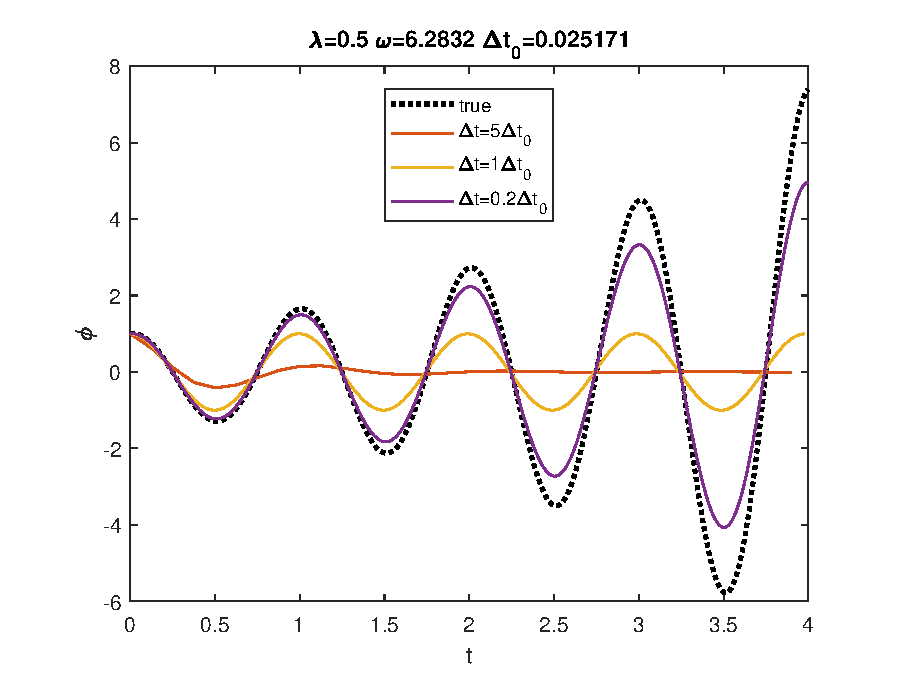
\includegraphics[width=0.45\linewidth]{hw1/backward_1}
    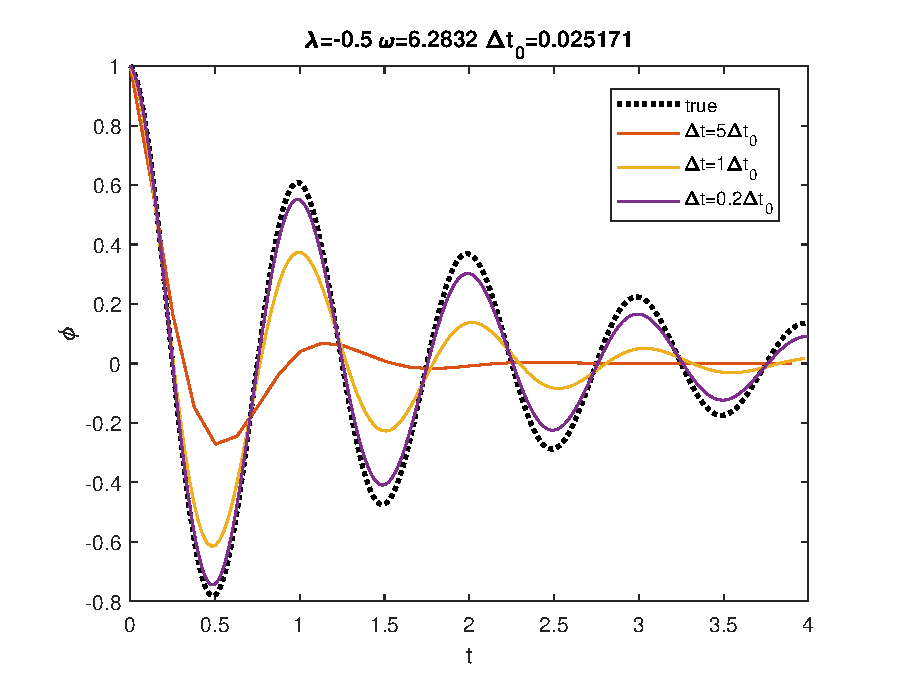
\includegraphics[width=0.45\linewidth]{hw1/backward_2}
    \caption{Different settings of backward difference scheme}
    \label{fig:backward}
\end{figure}
In figure \ref{fig:backward}, smaller amplitudes are present in all three schemes. When step is too large, the solution diverges from true solution.

\section{}
Modify the code (\verb|AStabilityConvergence_ODE_FT.m| and make it work for trapezoidal differencing schemes. Choose different $\Delta t$ and compare which one leads to the best convergence, which ones leads to unstable solution (you may refer to the matlab code provided). In this case, try positive $\lambda$.

\begin{figure}[!htbp]
    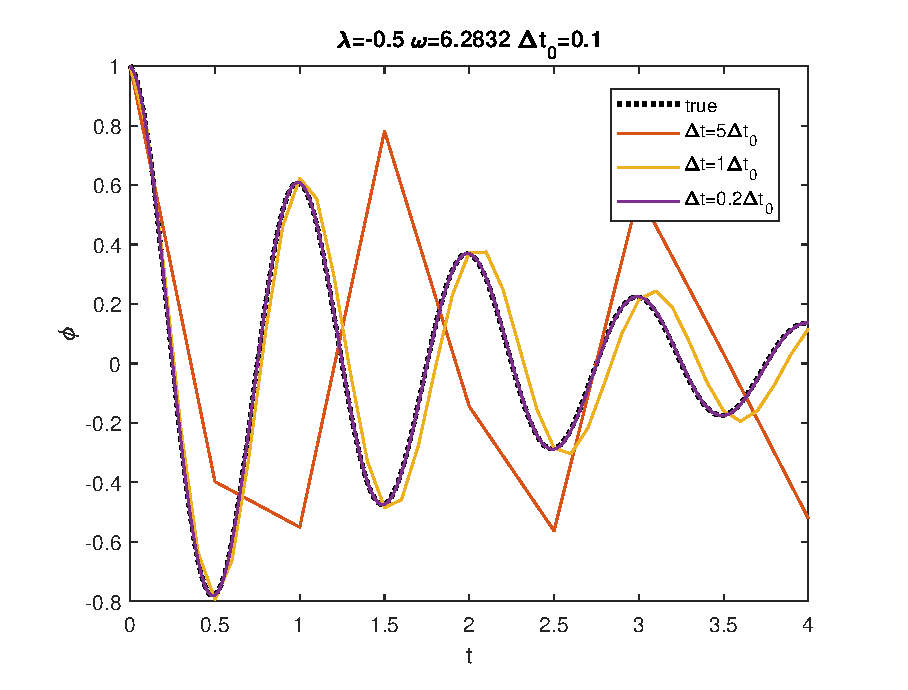
\includegraphics[width=0.45\linewidth]{hw1/trapezoidal_1}
    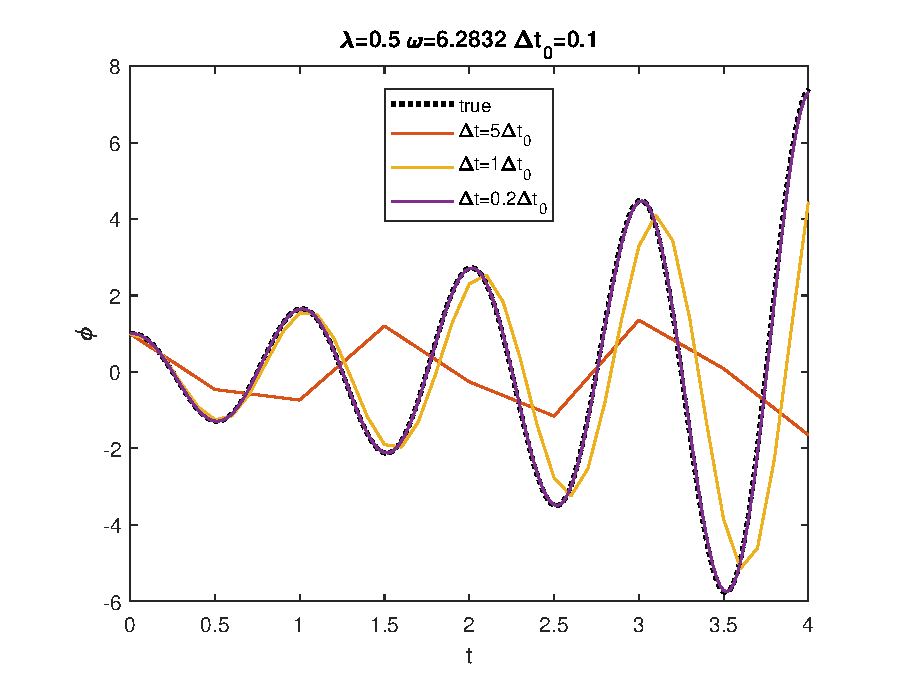
\includegraphics[width=0.45\linewidth]{hw1/trapezoidal_2}
    \caption{Different settings of trapezoidal difference scheme}
    \label{fig:trapezoidal}
\end{figure}
In figure \ref{fig:trapezoidal}, phase delays are present in all three schemes. When step is too large, the solution diverges from true solution.

\section{}
Compare with forward, backward and trapezoidal schemes, and discuss what you find.

In all three schemes, large step all leads to divergence. A small step is typically necessary for all difference schemes.